\chapter{Workflow Model}
\label{chapter-WorkflowModel}

This chapter presents the semantics and syntax of the workflow model that is
the foundation for the software that has been developed as part of this thesis.

\section{Semantics}

\subsection{Activities and Transitions}

The workflow model is activity-based. The activities that are to be completed
throughout the workflow and the transitions between them are mapped to the
nodes and edges of a directed graph. This choice was made to faciliate the
application of the Graph-Oriented Programming paradigm for the implementation
of the software component that is discussed in
Chapter~\ref{chapter-DesignAndImplementation}. Using a directed graph as the
foundation for the workflow model makes it possible to define the syntax of
the workflow description language using the formalism of graph grammars (see
Section~\ref{section-Syntax}).

\subsubsection{Graph Traversal and Execution Strategy}

The execution of a workflow starts with the graph's only \emph{Start} node. A
graph may have one or more \emph{End} nodes that explicitly terminate the
workflow execution.

After a node has finished executing, it can activate one or more of its
possible outgoing nodes. Activation adds a node to a set of nodes that
are waiting for execution. During each execution step, a node from this set
is executed. When the execution of a node has been completed, the node is
removed from the set.

The workflow execution is implicitly terminated when no nodes are activated
and no more nodes can be activated (see the \emph{Implicit Termination}
workflow pattern from \cite{BK03} that was discussed in Section
\ref{section-WorkflowPatterns}).

\subsection{State and Workflow Variables}

The workflow model supports state through the concept of workflow variables.
Such a variable can either be requested as user input (from an \emph{Input}
node) or be set and manipulated through the \emph{VariableSet},
\emph{VariableAdd}, \emph{VariableSub}, \emph{VariableMul}, \emph{VariableDiv},
\emph{VariableIncrement}, and \emph{VariableDecrement} nodes.

While a \emph{VariableSet} node may set the value of a workflow variable to
any type that is supported by the underlying programming language, the other
variable manipulation nodes only operate on numbers.

Variables are bound to the scope of the thread in which they were defined.
This allows parallel threads of execution to use variables of the same name
without side effects.

\subsubsection{Wait States}

When the execution of a workflow reaches an \emph{Input} node (see above),
the execution is suspended until such time when the user input has been
provided and the execution can be resumed.

\subsection{Control Flow}

The control flow semantics of the workflow model draws upon the workflow
patterns from \cite{BK03} that were discussed in Section
\ref{section-WorkflowPatterns}. The \emph{Sequence}, \emph{Parallel Split},
\emph{Synchronization}, \emph{Exclusive Choice}, \emph{Simple Merge},
\emph{Multi-Choice}, \emph{Synchronizing Merge}, and \emph{Discriminator}
workflow patterns are all directly supported by the workflow model.

\emph{Exclusive Choice} and \emph{Multi-Choice} nodes have branching
conditions attached to them that operate on workflow variables to make their
control flow decisions.

\subsection{Action Nodes and Service Objects}

So far we have only discussed nodes that control the flow and that can
manipulate workflow variables. We are still missing a type of nodes that
actually performs an activity. This is where the \emph{Action} node comes
into play.

When the execution of a workflow reaches an \emph{Action} node, the
business logic of the attached \emph{service object} is executed. Service
Objects ''live'' in the domain of the application into which the workflow
engine is embedded. They have read and write access to the workflow variables
to interact with the rest of the workflow.

\subsection{Sub-Workflows}

The workflow model supports sub-workflows to break down a complex workflow
into parts that are easier to conceive, understand, maintain, and which can
be reused.

A sub-workflow is started when the respective \emph{Sub-Workflow} node is
reached during workflow execution. The execution of the parent workflow is
suspended while the sub-workflow is executing. It is resumed once the
execution of the sub-workflow has ended.

\section{Syntax}
\label{section-Syntax}

\subsection{Graph Structure}

Graph Grammars are a formalism for the specification of visual languages. In
the following, we will use the \emph{reserved graph grammar} variant presented
by Zhang et al. in \cite{DQZ01}. It \emph{allows left-hand and right-hand
graphs of a production to have an arbitrary number of nodes and edges}. This
feature makes the graph grammars more expressive. A node in these graphs is a
two-level structure: a so-called \emph{super vertex} contains named vertices,
\emph{T (top)}, \emph{B (bottom)}, \emph{L (left)}, \emph{R (right)}. The
names correspond to the position of the vertex in the super vertex.

Figures \ref{figure-grammar-Axiom} to \ref{figure-grammar-Discriminator} show
the graph rewriting rules (productions) that make up the grammar for our
workflow model.

The \emph{Axiom} grammar rule shown in Figure~\ref{figure-grammar-Axiom}
expresses that an empty graph (left-hand side) can be transformed into a
graph that contains three nodes: a \emph{Start} node that has a
\emph{Statement} node as its only outgoing node, which in turn has an
\emph{End} node as its only outgoing node.

The \emph{Reduction} grammar rule shown in
Figure~\ref{figure-grammar-Reduction} expresses that a \emph{Statement} node
can be added to another \emph{Statement} node.

\begin{figure}[htb]
  \begin{minipage}{0.45\textwidth}
    \begin{center}
      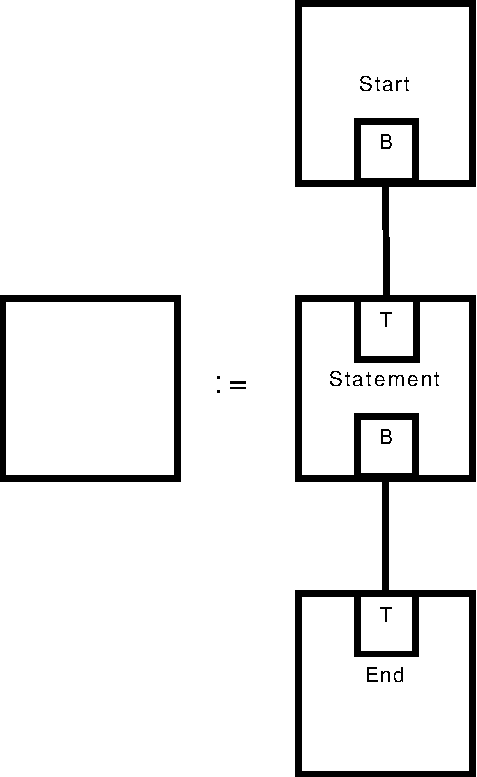
\includegraphics[width=4cm]{figures/grammar/axiom}\\[5mm]
      \caption[The \emph{Axiom} grammar rule]{Axiom}
      \label{figure-grammar-Axiom}
    \end{center}
  \end{minipage}
  \hfill
  \begin{minipage}{0.45\textwidth}
    \begin{center}
      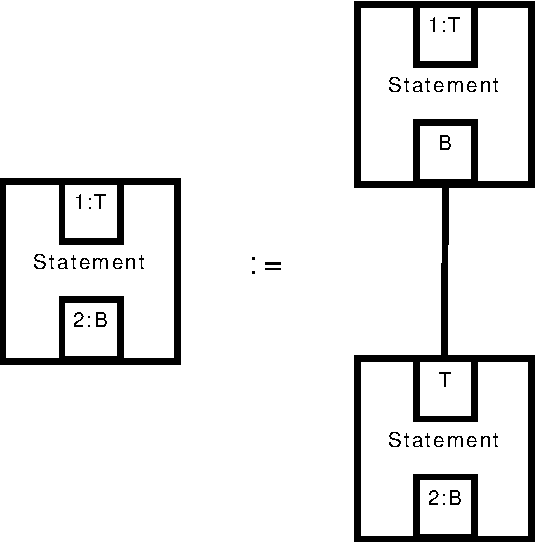
\includegraphics[width=4cm]{figures/grammar/reduction}\\[5mm]
      \caption[The \emph{Reduction} grammar rule]{Reduction}
      \label{figure-grammar-Reduction}
    \end{center}
  \end{minipage}
\end{figure}

\begin{figure}[htb]
  \begin{minipage}{0.45\textwidth}
    \begin{center}
      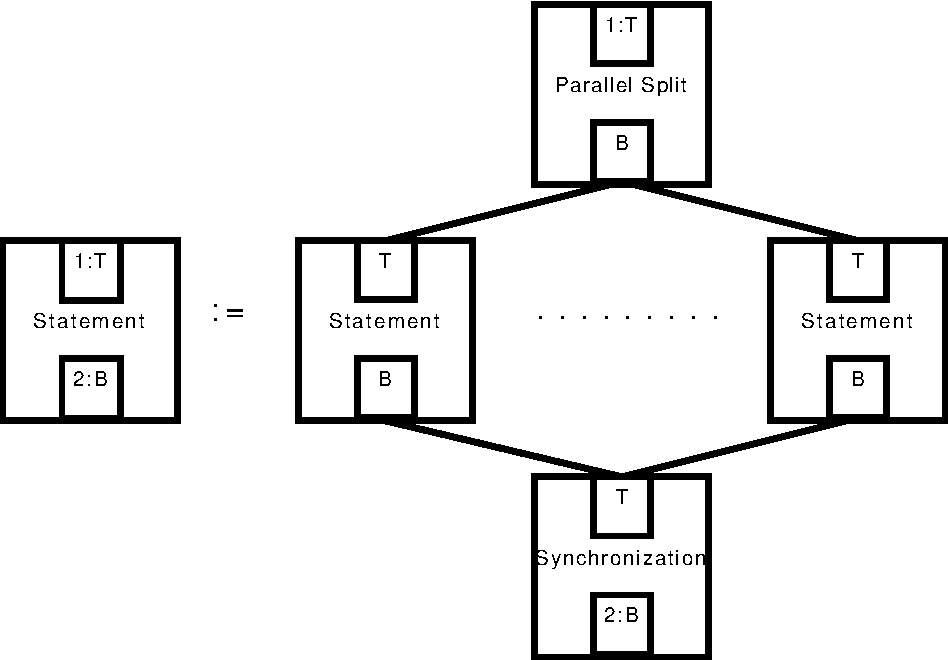
\includegraphics[width=7cm]{figures/grammar/and}\\[5mm]
      \caption[The \emph{AND} grammar rule]{AND}
      \label{figure-grammar-AND}
    \end{center}
  \end{minipage}
  \hfill
  \begin{minipage}{0.45\textwidth}
    \begin{center}
      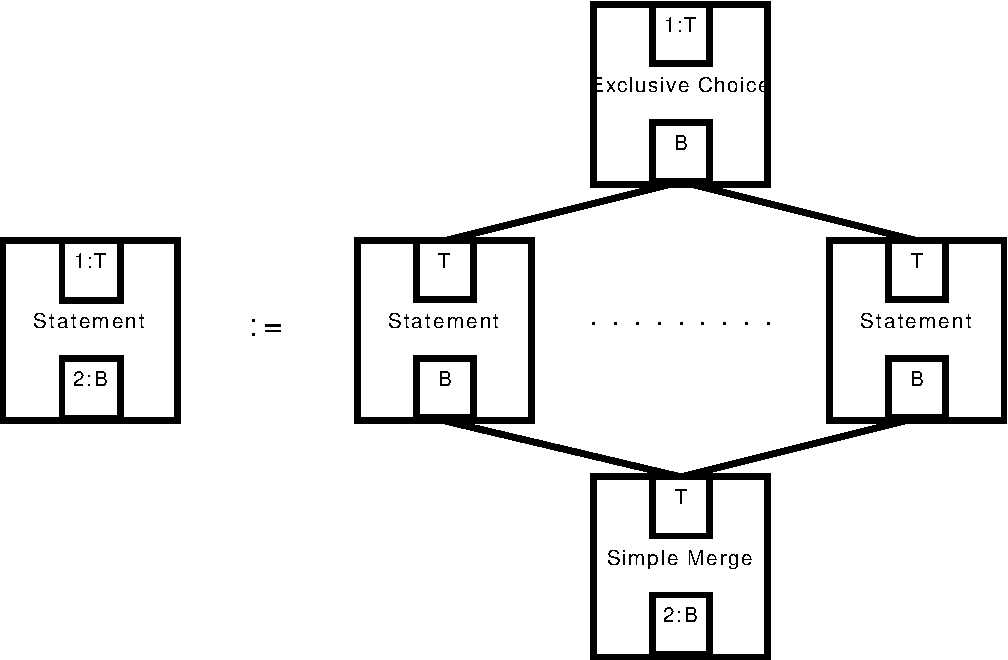
\includegraphics[width=7cm]{figures/grammar/xor}\\[5mm]
      \caption[The \emph{XOR} grammar rule]{XOR}
      \label{figure-grammar-XOR}
    \end{center}
  \end{minipage}
\end{figure}

A \emph{Statement} node can either be replaced by applying the grammar rules
shown in Figure~\ref{figure-grammar-AND} to \ref{figure-grammar-Discriminator}
or by replacing it with a node of type \emph{Action}, \emph{End}, \emph{Input},
\emph{Sub-Workflow}, \emph{VariableSet}, \emph{VariableAdd}, \emph{VariableSub},
\emph{VariableMul}, \emph{VariableDiv}, \emph{VariableIncrement}, and
\emph{VariableDecrement}.

\begin{figure}[htb]
  \begin{minipage}{0.45\textwidth}
    \begin{center}
      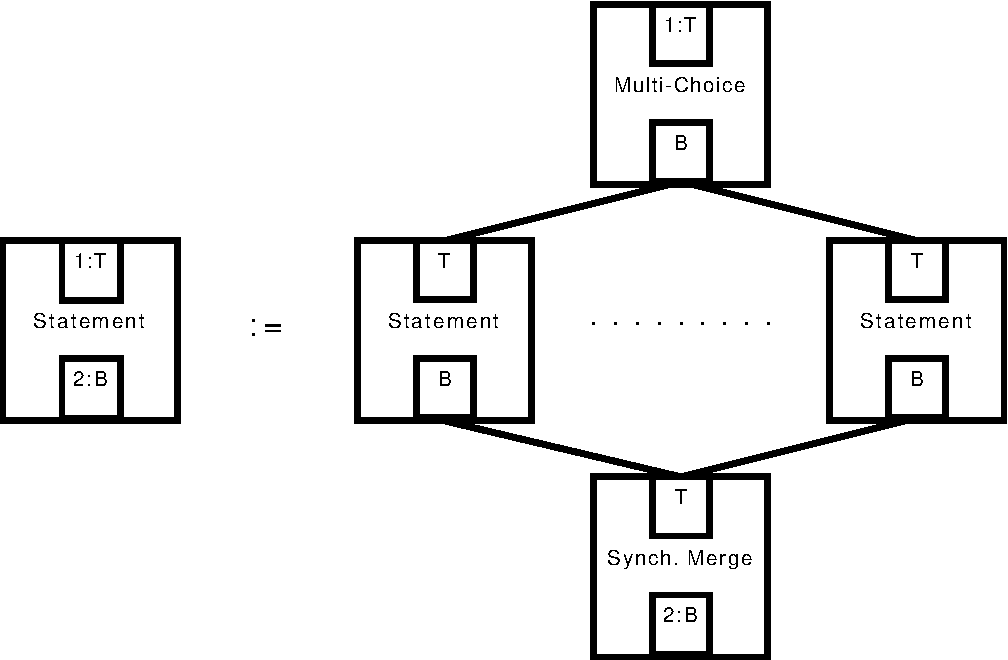
\includegraphics[width=7cm]{figures/grammar/or}\\[5mm]
      \caption[The \emph{OR} grammar rule]{OR}
      \label{figure-grammar-OR}
    \end{center}
  \end{minipage}
  \hfill
  \begin{minipage}{0.45\textwidth}
    \begin{center}
      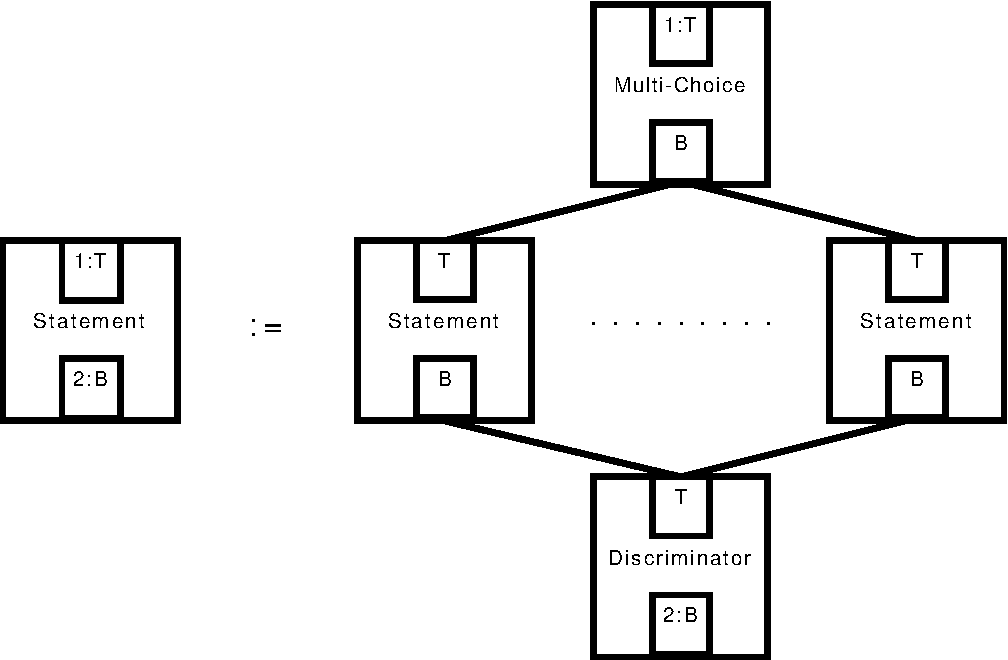
\includegraphics[width=7cm]{figures/grammar/discriminator}\\[5mm]
      \caption[The \emph{Discriminator} grammar rule]{Discriminator}
      \label{figure-grammar-Discriminator}
    \end{center}
  \end{minipage}
\end{figure}

\subsection{Conditions}

The conditions that can be used with branching and input nodes are expressions
built using the following constructs: \emph{Not}, \emph{And}, \emph{Or},
\emph{Xor}, \emph{IsAnything}, \emph{IsArray}, \emph{IsBool}, \emph{IsTrue},
\emph{IsFalse}, \emph{IsFloat}, \emph{IsInteger}, \emph{IsEqual},
\emph{IsNotEqual}, \emph{IsGreaterThan}, \emph{IsEqualOrGreaterThan},
\emph{IsLessThan}, \emph{IsEqualOrLessThan}, \emph{IsObject}, and
\emph{IsString}.

The examples in Appendix~\ref{section-ConditionClasses} show the syntax using
which these constructs can be combined to form condition expressions.

\section{Summary}

This chapter used the workflow patterns to describe the semantics and a graph
grammar to define the syntax of the workflow model that is the foundation for
the software that has been developed as part of this thesis.

The workflow model can be extended, for instance, with support for more
workflow patterns, by adding the respective node types.
